\section{Content Creation [L]}
Die Inhaltserstellungs-Funktion ist die Kernfunktion des Projekts. Die Content Creation definiert ein 3D-Portfolio. Ziel ist ein einfacher und intuitiver Konfigurationsprozess für ein 3D-Portfolios. 

\subsection{Datenstruktur}
Die 3D-Ausstellungen lassen sich durch Daten definieren. Die Daten werden bei der Content Creation vom*n Benutzer*in konfiguriert. 

\begin{figure}[ht]
    \centering
    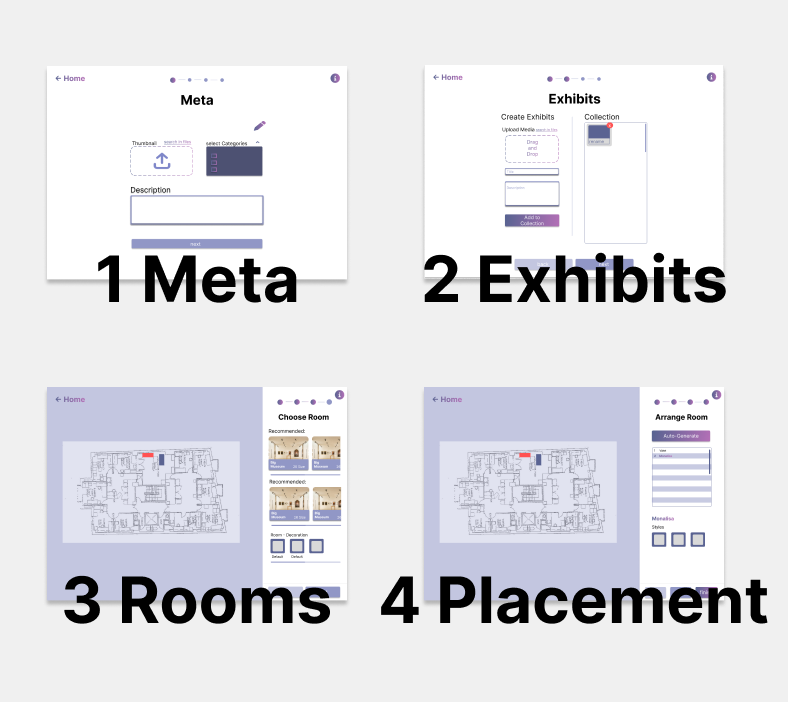
\includegraphics[scale=0.4]{pics/CreateCreation4Categories.png}
    \caption{Inhaltserstellungstool}
    \label{fig:impl:creation:fourCategoires}
\end{figure}

\subsubsection{Kategorie}
\label{sec:wizard:categories}
Die Datenstruktur des Protfolios lässt sich logisch in vier Kategorien (siehe Abbildung \ref{fig:impl:creation:fourCategoires}) teilen. 
Die Kategorien sind:
\begin{compactitem}
\item Metadaten - Die Metadaten sind beschreibende Daten des Portfolio, dazu gehören Name, zugehörige Kategorien, eine Beschreibung und ein Thumbnail.
\item Ausstellungsstücke - Die Ausstellungsstücke werden in dem 3D-Portfolio präsentiert. Die Ausstellungsstücke, Film-, Foto- und 3D Dateien,  werden vom*von Benutzer*in hochgeladen und mit Zusatzinformation wie Namen und Beschreibung ergänzt. 
\item Raumdaten - Raumdaten bestehen aus virtuellen 3D-Daten des Raumes und weiteren Konfigurationsdaten wie den Positionen, an denen Ausstellungsstücke im Raum platziert werden können. Der Grundriss des Raumes kann jede beliebige Form besitzen. 
\item Ausstellungsplatzierungsdaten - Mit diesen Daten werden die Ausstellungsstücke mit dem virtuellen Raum verbunden. Außerdem ist in den Ausstellungsplatzierungsdaten die Dimension eines Ausstellungsstückes enthalten. Jedes Position besitzt eine definierbare Sockelart. 
\end{compactitem}

\paragraph{Ausprägungen}
In der SPA werden die vier Kategorien durch Klassen (siehe Abbildung \ref{fig:impl:creation:dataclasses}) definiert. 

\begin{figure}[ht]
    \centering
    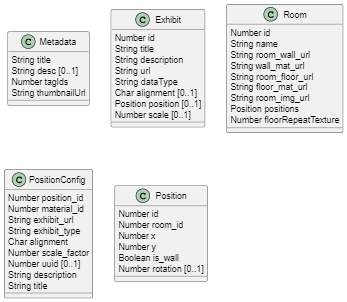
\includegraphics[scale=0.9]{pics/content_creation_classes.png}
    \caption{Inhaltserstellung Datenklassen}
    \label{fig:impl:creation:dataclasses}
\end{figure}

\subsection{GUI}
\subsubsection{Profilepage}
Auf der Profileseite (siehe Abbildung \ref{fig:impl:sign:profile}) sieht der*die Benutzer*in userspezifische Informationen wie den Profilnamen, das Profilfoto und die erstellten Ausstellungen. Zusätzlich kann der*die Benutzer*in hier neue Ausstellungen anlegen und bereits erstellte Ausstellungen löschen.

\begin{figure}
  \centering
  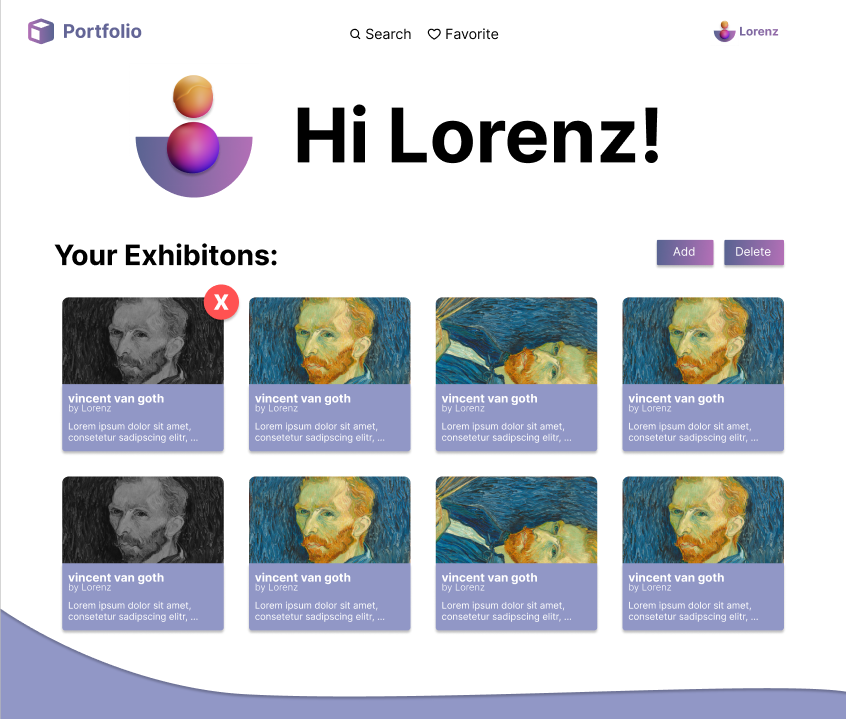
\includegraphics[scale=0.5]{pics/profilepage.png}
  \caption{Profilepage}
  \label{fig:impl:sign:profile}
\end{figure}

\paragraph*{Add Button}
Der Content-Creation-Prozess beginnt damit, dass der Add-Button auf der Profileseite gedrückt wird. Danach wird der*die Benutzer*in zu dem Content-Creation-Tool auf der SPA weitergeleitet. Dort startet er*sie den Konfigurationsprozess mit dem Metadaten-Formular.


\subsubsection{Formulare}
Die Datensammlung wurde nach vier Formularen, die jeweils einer der vier Datenkategorien (siehe im Abschnitt \ref{sec:wizard:categories}) sammeln, aufgeteilt. Das hat das Ziel, dass der*die Benutzer*in sich im Konfigurationsprozess nur mit jeweils einer Portfolio-Daten-Kategorie beschäftigen muss und nicht überfordert wird. Dabei wurde sich am \emph{Wizard-UI-Pattern} (mehr dazu im Unterkapitel \ref{sec::contentcreation::wizard} auf der Seite \pageref{sec::contentcreation::wizard}) orientiert.


\paragraph{Metadaten-Formulare}
Im Metadaten-Formular werden die Metadaten der Ausstellung gesammelt.


Dabei wurden für die Sammlung der Namen, Beschreibungen und Kategorien der Ausstellung die reaktiven Formulare von Angular und für das Vorschaubild der Ausstellung die eigene Upload-Komponente benutzt. (siehe Abschnitt Upload \ref{sec:wizard:upload}).


\paragraph{Exhibit-Formular}
Im Exhibit-Formular lädt der*die Benutzer*in seine*ihre digitalen Ausstellungsstück hoch.

Beim Upload gibt es Einschränkungen. Ausstellungstücke können nur hochgeladen werden, wenn ihre Datengröße kleiner als 50 MB ist und ihr Filetyp unterstützt wird. Es werden für 3D-Dateien GLTF-Files, für Video-Dateien MP4 und für Photo-Dateien JPG und PNG unterstützt (siehe Abschnitt Upload \ref{sec:wizard:upload})

\paragraph{Raum-Formular}
Im Raumformular wählt der*die User*in zwischen den vordefinierten Grundrissen aus.

In einer 3D-Ansicht neben den Auswahlmöglichkeiten sieht man eine Vorschau, wie der ausgewählte Raum ohne Ausstellungstücke aussieht. 
Ein Grundriss definiert auch die möglich Positionen der Ausstellungsstücke und damit auch die Anzahl wie viele Ausstellungsstücke jeweils in einem Raum seinen können. Dem*Der User*in werden die Räume vorgeschlagen, nachdem wie viele Ausstellungsstücke er*sie im vorherigen Formualre Exhibit-Formular kreiert hatte. 

\paragraph{Ausstellungs-Platzierungs-Formular}
Im Ausstellungs-Platzierungs-Formular werden die hochgeladenen Ausstellungstücke mit dem Grundriss der Ausstellung verbunden.  In einer 3D-Ansicht neben den Auswahlmöglichkeiten sieht man eine Vorschau, wie der Raum mit den Ausstellungstücke aussieht. 

Ein Grundriss hat dabei mehrere Positionen. An diesen können Ausstellungsobjekte platziert werden. Die Ausstellungsstücke können manuell und automatisch an der Position platziert werden.
Dabei wird nach der Ausstellungsstück-Type unterschieden: 3D-Datei oder Photo und Video-Datei. Nach dem Datei-Type des Ausstellungstücks wird an der Position entweder ein Sockel oder ein Bilderrahmen mit dem Ausstellungstück erschaffen. Der Typ des Sockels und des Bilderrahmens können geändert werden.
Die Größe eines 3D-Ausstellungsstückes wird normalisiert, damit alle Ausstellungstücke gleich groß sind und dem*der User*in wird die Möglichkeit gegeben, diese Größe noch zu ändern.

\paragraph{Userinterface-Struktur / Wizard Design Pattern [L]}
\label{sec::contentcreation::wizard}
Im Projekt wurde das Wizard-UI-Pattern benutzt, um den Konfigurationsprozess des Portfolios einfacher zu gestalten.

\paragraph*{Wizard Begriffserklärung [L]}
Der Begriff "\emph{Wizard}" in der Softwareentwicklung, kommt ursprünglich von Systemadministratoren, welche bei komplizierten Installationsprozessen halfen oder ganz übernahmen. Mit der Zeit änderte sich der Begriff zu Software-Assistenten-Programmen, welche dem*der User*in dabei unterstützten, die Software zu konfigurieren. \cite[Ursprung des Begriffs Wizard]{OrigionOfWizards}

\paragraph{Wizard-UI-Pattern [L]}
Im Web-Bereich gibt es in der Regel zwei Arten Dateneintragungen zu verarbeiten.

Formulare und Wizards. Ein Wizard ist eine eigene kleine Applikation, die den*die Benutzer*in durch eine Folge von Formularen führt und gegebenenfalls beim Ausfüllen unterstützt. Je nach den Eingaben können Wizards die Reihenfolge oder die Formulare ändern.\cite[Wizards: Definition and Design Recommendations]{WizradsDefinitionAndRecommandation}

\paragraph{Umsetzung des Wizards [L]}
Für die Umsetzung des Wizards wurde die Angular Material Komponente Mat-Stepper benutzt. Sie bietet eine solide Basis für den Wizard. Content kann sequentiell dargestellt werden, während dem*der User*in der aktuelle Status des Wizards durch eine Navigationsleiste angezeigt wird (siehe Abbildung \ref{fig:impl:creation:mathorziontalstepper}). \cite{amStepper}

\begin{figure}
    \centering
    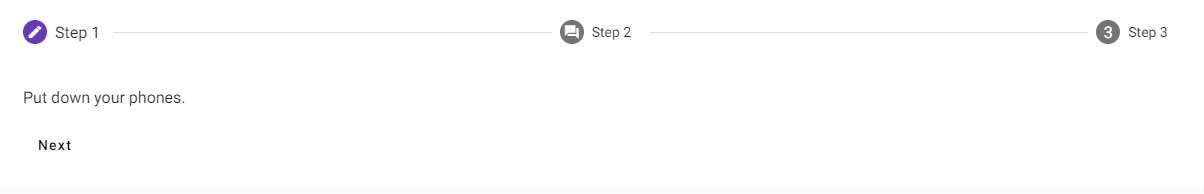
\includegraphics[scale=0.5]{pics/mathorziontalstepper.png}
    \caption{Angular Material: horizontaler Stepper \cite{amStepper}}
    \label{fig:impl:creation:mathorziontalstepper}
\end{figure}

\subsection{Upload}
\label{sec:wizard:upload}
Die Dateien-Hochlade-Komponente wurde mit dem Gedanken entwickelt, hoch modular und anpassungsfähig zu sein. Denn die Hochlade-Funktion wird öfters im Projekt gebraucht.

Bei der Komponente sind akzeptable Filetypen und Filegrößen einzustellen, werden die gesetzten Anforderungen an Filetypen und Filegrößen von den hochzuladenden Daten nicht erfüllt, so werden diese auch nicht hochgeladen und die Komponente gibt eine Fehlermeldung.
Bei einem erfolgreichen Hochladeprozess bekommt die Komponente eine URL vom Server. Unter der URL ist die hochgeladene Datei erreichbar.








\subsection{Erledigte Userstories [L]}
In dem Entwicklungsprozess der Content-Creation-Tool wurden folgende Userstories vollendet:
\begin{compactenum}
    \item  Als User*in will ich eine Profil-Unterseite haben, auf der ich userrelevante Informationen angezeigt bekomme. Akzeptanzkriterien:
    \begin{compactitem}
        \item userrelevante Informationen, die angezeigt werden, sind:
        \begin{compactitem}
            \item Name
            \item Profilfoto
            \item Erstellte Ausstellungen        
        \end{compactitem}
        \item Der*Die User*in kann dort seine Ausstellungen löschen.        
    \end{compactitem}
    \item Als User*in will ich bei der Erstellung einer Ausstellung zwischen verschiedenen Templates wählen können, um diese auf einfache Weise zu individualisieren. Akzeptanzkriterien:
    \begin{compactitem}
        \item Der*Die User*in kann keine Templates erstellen.
        \item Der*Die User*in kann manuell die Podeste für jede Datei zwischen mehrere vorgefertigten auswählen und für den Boden + Wand ein Pattern hochladen
    \end{compactitem}
    \item Als User*in will ich meine Daten auf den Server laden, um diese jederzeit innerhalb einer Ausstellung platzieren und integrieren zu können. Akzeptanzkriterien:
    \begin{compactitem}
        \item Unterstützte Dateien (Bilder-, Audio-, Video-, 3D-Dateien)
        \item Uploadmöglichkeiten:
        \begin{compactitem}
            \item Im Ordner auswählen.
        \end{compactitem}
        \item Dateigrößenlimit: 50MB
        \item Dateityp Limit: nur Standardformate (Bilder: JPG, PNG, etc.; etc.; …)
        \item Fehlermeldung bei falschem Upload
    \end{compactitem}
    \item  Als User*in will ich, dass meine Daten automatisch als Ausstellungsstücke in der Ausstellung angeordnet werden, damit die Nutzung für persönliche Bereiche unkompliziert möglich ist. Akzeptanzkriterien:
    \begin{compactitem}
        \item Falls dies nicht möglich ist, soll eine Fehlermeldung angezeigt werden
    \end{compactitem}
    \item Als User*in möchte ich die Reihenfolge und Platzierung meiner Werke innerhalb der Ausstellung adaptieren können. Akzeptanzkriterien:
    \begin{compactitem}
        \item Die Werke sollen zwischen vordefinierten Plätzen tauschbar sein.
    \end{compactitem}
    \item Als User*in möchte ich meine Ausstellung abspeichern und löschen können. Akzeptanzkriterien:
    \begin{compactitem}
        \item Die Daten im Bezug auf die Ausstellungen werden auf dem Server gespeichert.
        \item Bevor die Ausstellung gelöscht wird, soll ein Warnhinweis angezeigt werden, welcher noch bestätigt werden muss.
    \end{compactitem}
    \item Als Benutzer*in möchte ich meinen Ausstellungen Tags zuordnen können, damit diese leichter gefunden werden können. Akzeptanzkriterien:
    \begin{compactitem}
        \item Tags werden beim erstellen der Ausstellung aus einen vordefinierten Tag-Pool ausgewählt.
    \end{compactitem}
\end{compactenum}
 








%%\section{3D-Portfolio-Gallery Konfigurationstool [L]} \label{Konfigurationstool}
%%\setauthor{Litzlbauer Lorenz}
%%
%%Die Inhaltserstellung-Funktion ist die Kernfunktion des Projekts. Die Content Creation definiert ein 3D-Portfolio. Ziel ist ein einfacher und intuitiver Konfigurationsprozess für ein 3D-Portfolios. 
%%yyy Im Entwicklungsprozess wurden viele Entscheidungen getroffen, die auf das ganze Projekt Einfluss hatten. Z.B. wurde eine Art der Datenrepräsentation der 3D-Portfolios und die Darstellungsweise der Daten in der 3D-View entwickelt.
%%
%%In diesem Kapitel wird die Softwareentwicklung und der Prozess der Inhaltserstellung erklärt.
%%
%%\begin{figure}
%%    \centering
%%    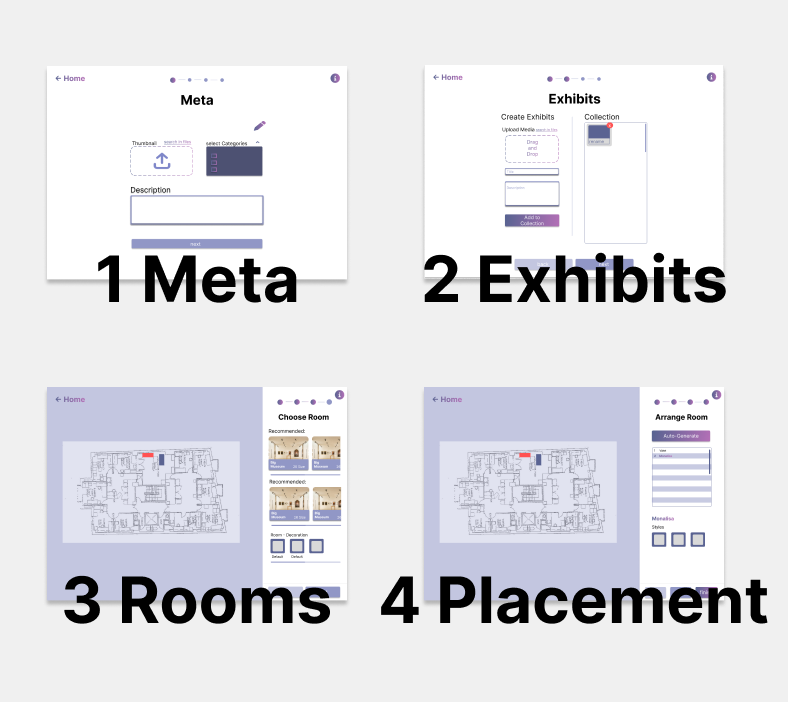
\includegraphics[scale=0.5]{pics/CreateCreation4Categories.png}
%%    \caption{Inhaltserstellungstool}
%%    \label{fig:impl:creation:fourCategoires}
%%\end{figure}
%%
%%\subsection{Überblick [L]}
%%Das Inhaltserstellungs-Tool besteht aus insgesamt vier Bereichen (siehe Abbildung \ref{fig:impl:creation:fourCategoires}), mit diesen werden Daten gesammelt, um das Portfolio zu erstellen und vielen Untersystemen (bestehend aus Komponenten, Klassen und Services siehe Unterkapitel \ref{sec::impl::contentcreation::UnterstuetzendeServicesUndKlassen} auf Seite \pageref{sec::impl::contentcreation::UnterstuetzendeServicesUndKlassen}) , die beim Erstellungsprozess helfen.
%%
%%Diese Unterseiten wurden aufgeteilt, damit der*die Benutzer*in sich im Konfigurationsprozess nur mit jeweils einer Portfolio-Daten-Kategorie beschäftigen muss und nicht überfordert wird. Dabei wurde sich  am \emph{Wizard-UI-Pattern} (mehr dazu im Unterkapitel \ref{sec::contentcreation::wizard} auf der Seite \pageref{sec::contentcreation::wizard}) orientiert.
%%
%%\subsection{Userinterface-Struktur / Wizard Design Pattern [L]}
%%\label{sec::contentcreation::wizard}
%%Im Projekt wurde das Wizard-UI-Pattern benutzt, um den Konfigurationsprozess des Portfolios einfacher zu gestalten. Dafür wurden die Konfigurationsdaten nach 4 Kategorien aufgeteilt und für jede eine eigene Unterseite (siehe Abbildung \ref{fig:impl:creation:fourCategoires}) entworfen.
%%
%%Die Kategorien sind:
%%\begin{compactitem}
%%\item Metadaten - Die Metadaten sind beschreibende Daten für das Portfolio, dazu gehören Name, zugehörige Kategorien, eine Beschreibung und ein Thumbnail.
%%\item Ausstellungsstück - Die Daten des Ausstellungsstücks bestehen aus den vom User auf den Server geladenen Kunstwerken und Zusatzinformation wie Namen und Beschreibung.
%%\item Raumdaten - Raumdaten bestehen aus den virtuellen 3D-Daten des Raumes und weiteren Konfigurationsdaten wie den Positionen, an denen Ausstellungsstücke im Raum platziert werden können.
%%\item Ausstellungsplatzierungsdaten - Mit diesen Daten werden die Daten zu den Ausstellungsstücken und dem virtuellen Raum logisch verbunden.
%%\end{compactitem}
%%
%%\subsubsection*{Begriffserklärung [L]}
%%Der Begriff "\emph{Wizard}" in der Softwareentwicklung, kommt ursprünglich von Systemadministratoren, welche bei komplizierten Installationsprozessen halfen oder ganz übernahmen. Mit der Zeit änderte sich der Begriff zu Software-Assistenten-Programmen, welche dem*der User*in dabei unterstützten, die Software zu konfigurieren. \cite[Ursprung des Begriffs Wizard]{OrigionOfWizards}
%%
%%\subsubsection{Wizard-UI-Pattern [L]}
%%Im Web-Bereich gibt es in der Regel zwei Arten Dateneintragungen zu verarbeiten.
%%
%%Formulare und Wizards. Ein Wizard ist eine eigene kleine Applikation, die den*die Benutzer*in durch eine Folge von Formularen führt und gegebenenfalls beim Ausfüllen unterstützt. Je nach den Eingaben können Wizards die Reihenfolge oder die Formulare ändern.
%%
%%TODO: Bei Bedarf könnte hier mehr geschrieben werden. \cite[Wizards: Definition and Design Recommendations]{WizradsDefinitionAndRecommandation}
%%
%%\subsubsection{Implementation [L]}
%%Für die Implementation des Wizards wurde die Angular Material Komponente Mat-Stepper benutzt. Sie bietet eine solide Basis für den Wizard. Content kann sequentiell dargestellt werden, während dem*der User*in der aktuelle Status des Wizards durch eine Navigationsleiste angezeigt wird (siehe Abbildung \ref{fig:impl:creation:mathorziontalstepper}). \cite{amStepper}
%%
%%\begin{figure}
%%    \centering
%%    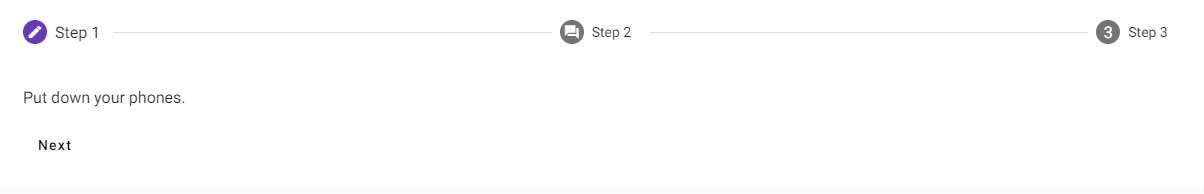
\includegraphics[scale=0.5]{pics/mathorziontalstepper.png}
%%    \caption{Angular Material: horizontaler Stepper \cite{amStepper}}
%%    \label{fig:impl:creation:mathorziontalstepper}
%%\end{figure}
%%
%%\subsection{4 Formularunterseiten [L]}
%%Nachdem die Angular Material Komponente Mat-Stepper für die Wizard-Funktionalität gewählt wurde, war der nächste Schritt, die vier Formularunterseiten des Wizards (siehe Abbildung \ref{fig:impl:creation:fourCategoires}) zu gestalten.
%%
%%In diesem Unterkapitel werden die Funktionalitäten und die Probleme bzw. Lösungen dieser Unterseiten beschrieben. 
%%
%%\subsubsection{Kommunikationsschnittstelle [L]}
%%Die Unterseiten sammeln Daten für die Erstellung des Portfolios. Die Kommunikationsschnittstellen der Unterseiten helfen dabei, dass die Unterseiten miteinander kommunizieren können. Dafür wurde das \emph{Observer-Design-Pattern} (siehe im Glossar \ref{txt:glos:observerDesignPattern} auf Seite \pageref{txt:glos:observerDesignPattern}) gewählt.
%%
%%In einer Dienstklasse, die durch Dependency Injection (siehe Unterkapitel \ref{DPI} auf Seite \pageref{DPI}) mit allen Unterseiten verbunden ist, befinden sich Observablen, die mit den Eingabefeldern der Unterseiten verbunden sind. Wenn auf den Unterseiten eine neue Dateneingabe geschieht, wird die Veränderung an die Dienstklasse weitergegeben. Die Unterseiten haben jeweils eine Datenklasse nach den Kategorien des Portfolios (siehe Abbildung \ref{fig:impl:creation:dataclasses}), in der die Daten gespeichert werden.
%%
%%\begin{figure}
%%    \centering
%%    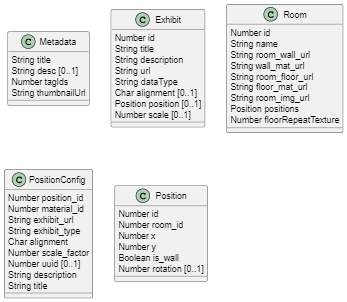
\includegraphics[scale=0.7]{pics/content_creation_classes.png}
%%    \caption{Inhaltserstellung Datenklassen}
%%    \label{fig:impl:creation:dataclasses}
%%\end{figure}
%%
%%In der Dienstklasse werden Veränderungen durch den SessionStorage (siehe Unterkapitel \ref{par:impl:usermanagment:WebStorage} auf Seite \pageref{par:impl:usermanagment:WebStorage}) gespeichert und an den Wizard Mat-Stepper weitergeleitet, um dort den Fortschritt des Konfigurationsprozesses anzuzeigen.
%%
%%Durch die Speicherung im SessionStorage kann der Konfigurationsprozess selbst bei einem Abbruch in der Zukunft nahtlos fortgesetzt werden.
%%
%%\subsubsection{Metadaten - Unterseite [L]}
%%Die Metadaten-Unterseite (siehe Abbildung \ref{fig:impl:creation:Metadaten_Unterseite}) wurde erstellt, um Metadaten wie den Namen, die Kategorien, das Vorschaubild und eine kurze Beschreibung zu der Ausstellung zu sammeln.
%%
%%Alphanumerische Daten wie der Name und die Beschreibung wurden mit Angular's reaktiven Formularen (siehe Kapitel \ref{par:impl:usermanagment:reactiveForms} auf Seite \pageref{par:impl:usermanagment:reactiveForms}) gesammelt.
%%
%%Das Vorschaubild wird hochgeladen mit der Dateien-Hochlade-Komponente (siehe Kapitel \ref{sec:impl:contentcreation:file-Upload} auf Seite \pageref{sec:impl:contentcreation:file-Upload}). Auf der Webapplikation wird die URL gespeichert, unter der die hochgeladene Datei zur Verfügung steht.
%%
%%\begin{figure}
%%    \centering
%%    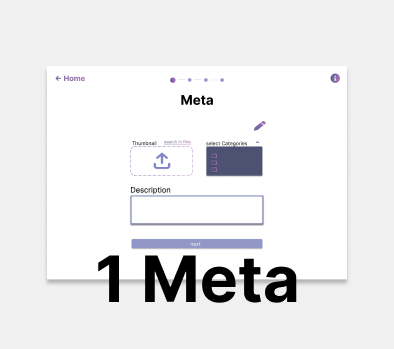
\includegraphics[scale=0.5]{pics/metadaten.png}
%%    \caption{Metadaten Unterseite}
%%    \label{fig:impl:creation:Metadaten_Unterseite}
%%\end{figure}
%%
%%\subsubsection{Ausstelungsstücke - Raum}
%%\subsection{Unterstützende Services und Klassen}
%%\label{sec::impl::contentcreation::UnterstuetzendeServicesUndKlassen}
%%\subsubsection{Dateien-Hochlade-Komponente [L]}
%%\label{sec:impl:contentcreation:file-Upload}
%%
%%TODO: Image vom der Komponente
%%
%%
%%\paragraph{Funktionalitäten und Implementierung [L]}
%%\paragraph{Hochlade Funktionalitäten des Servers [E]}
%%
%%
%%\subsubsection{Portfolio-Veröffentlichung-System [L]}